\section{Business Context}

\label{chap:business_context}

Based on the rules explained in \autoref{chap:SPITCH}, two main findings emerge. The first point is the main objective of the game: assemble a team of 11 players that will score as many points as possible on the upcoming match day. The second point is that the constraint placed on the players, the budget, can be converted to a player's total score. Regarding the first point, it is necessary to distinguish at what point the main goal of the game is achieved. There are three different angles to approach this: if only the problem itself is considered, the goal would be to put together the team that scores highest. Secondly, from a game perspective, it would be enough to field the best team of all competitors, i.e., to place first in the final ranking. Lastly, a purely economic objective would be to put together a team that makes a profit by ending in the profit zone at the end of the game. 

Past rankings show that even the first place of a matchday never achieves the whole number of points. Instead, the top ranks only reach 80 to 85\% of the maximum possible score. This paragraph aims to present an example for this claim. Therefore, the following screenshots from the 8th matchday of the 2021/22 Bundesliga season are evaluated. The first screenshot shows the top 10 ranking for this matchday. This screenshot indicates that the scores of the top managers differ only slightly.

\begin{figure}[H]
    \centering
    \fbox{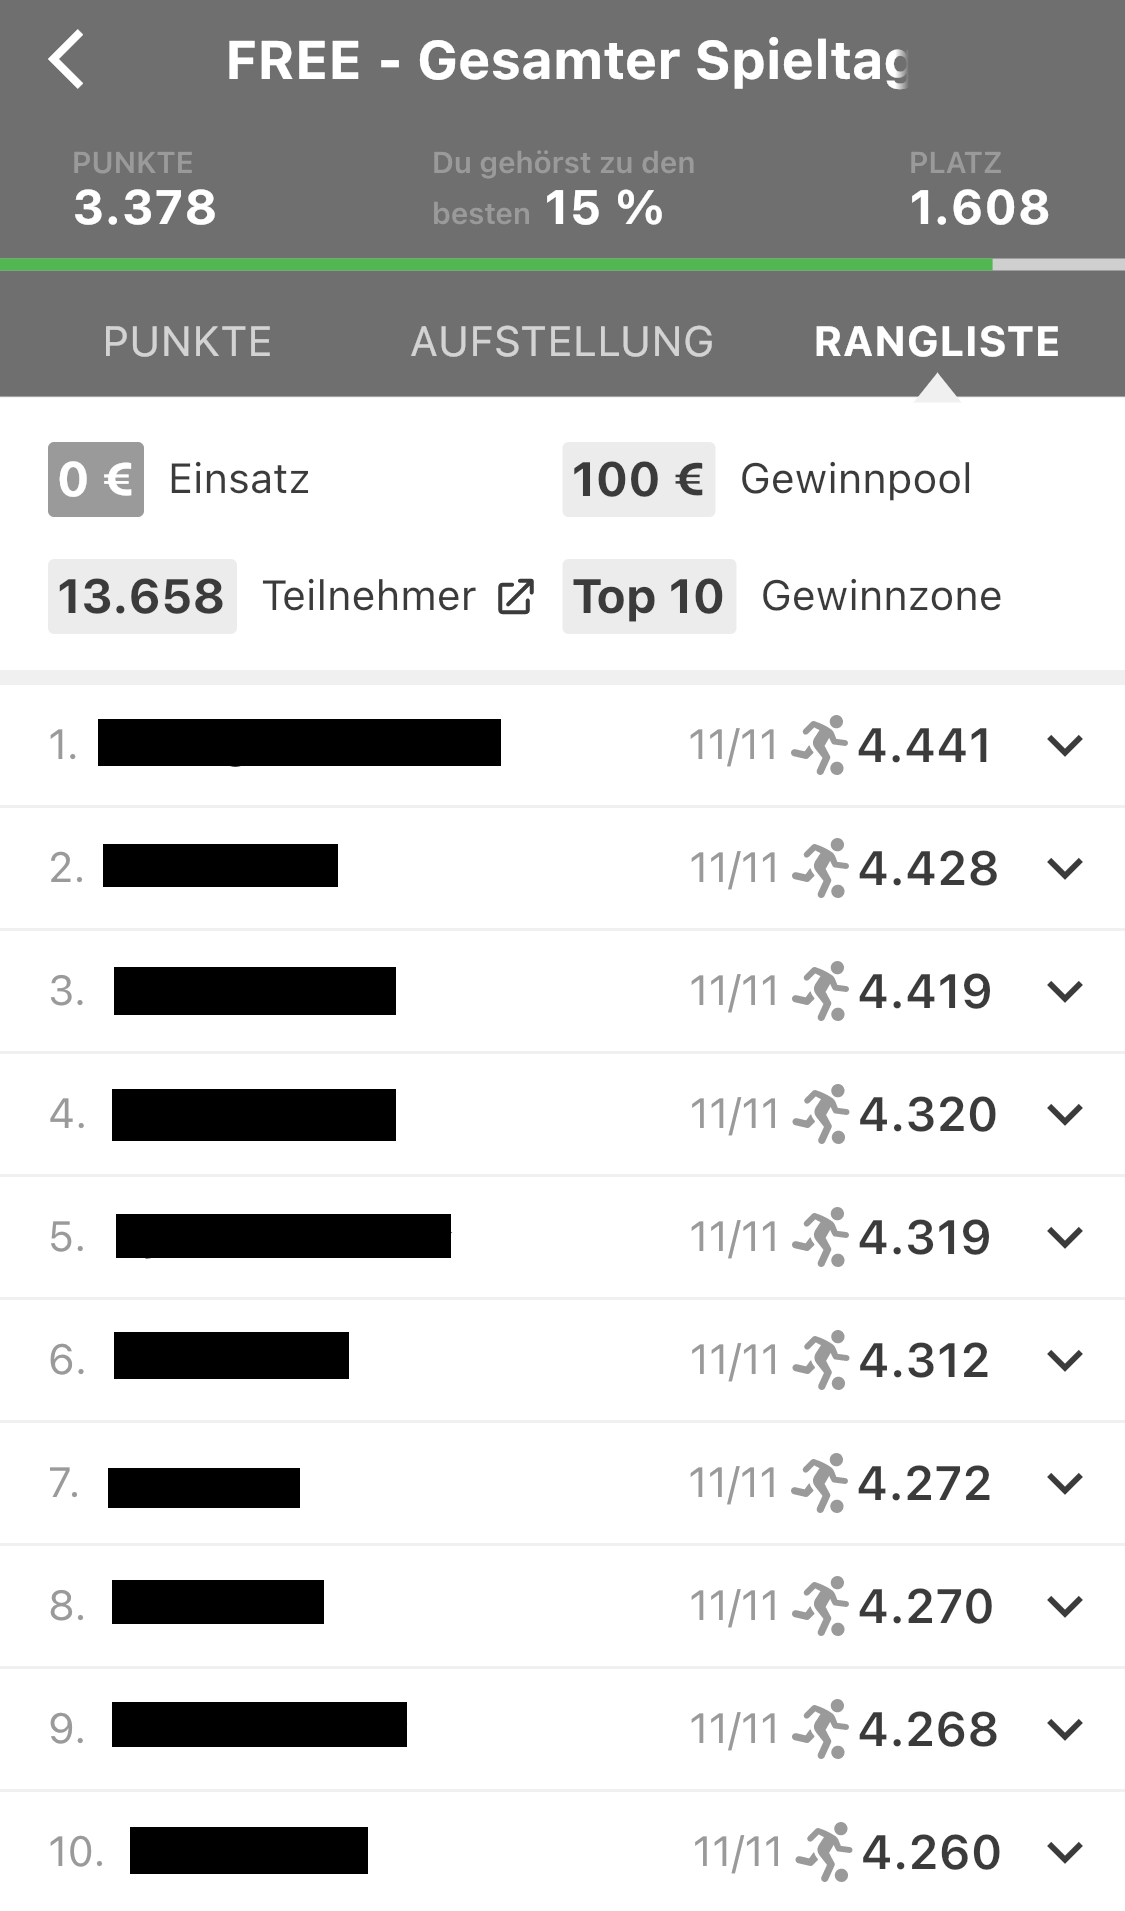
\includegraphics[width=7cm]{chapter/4_implementation/figures/ranking.png}}
    \captionsetup{justification=centering}
    \caption{Top 10 Ranking FREE Pitch, 8th matchday 2021/22}
    \label{fig:top-10}
\end{figure}

\clearpage Additionally, the following screenshots show the line-ups of the best three managers for this matchday. 

\begin{figure}[htp]
    \makebox[\textwidth][c]{
        \fbox{
            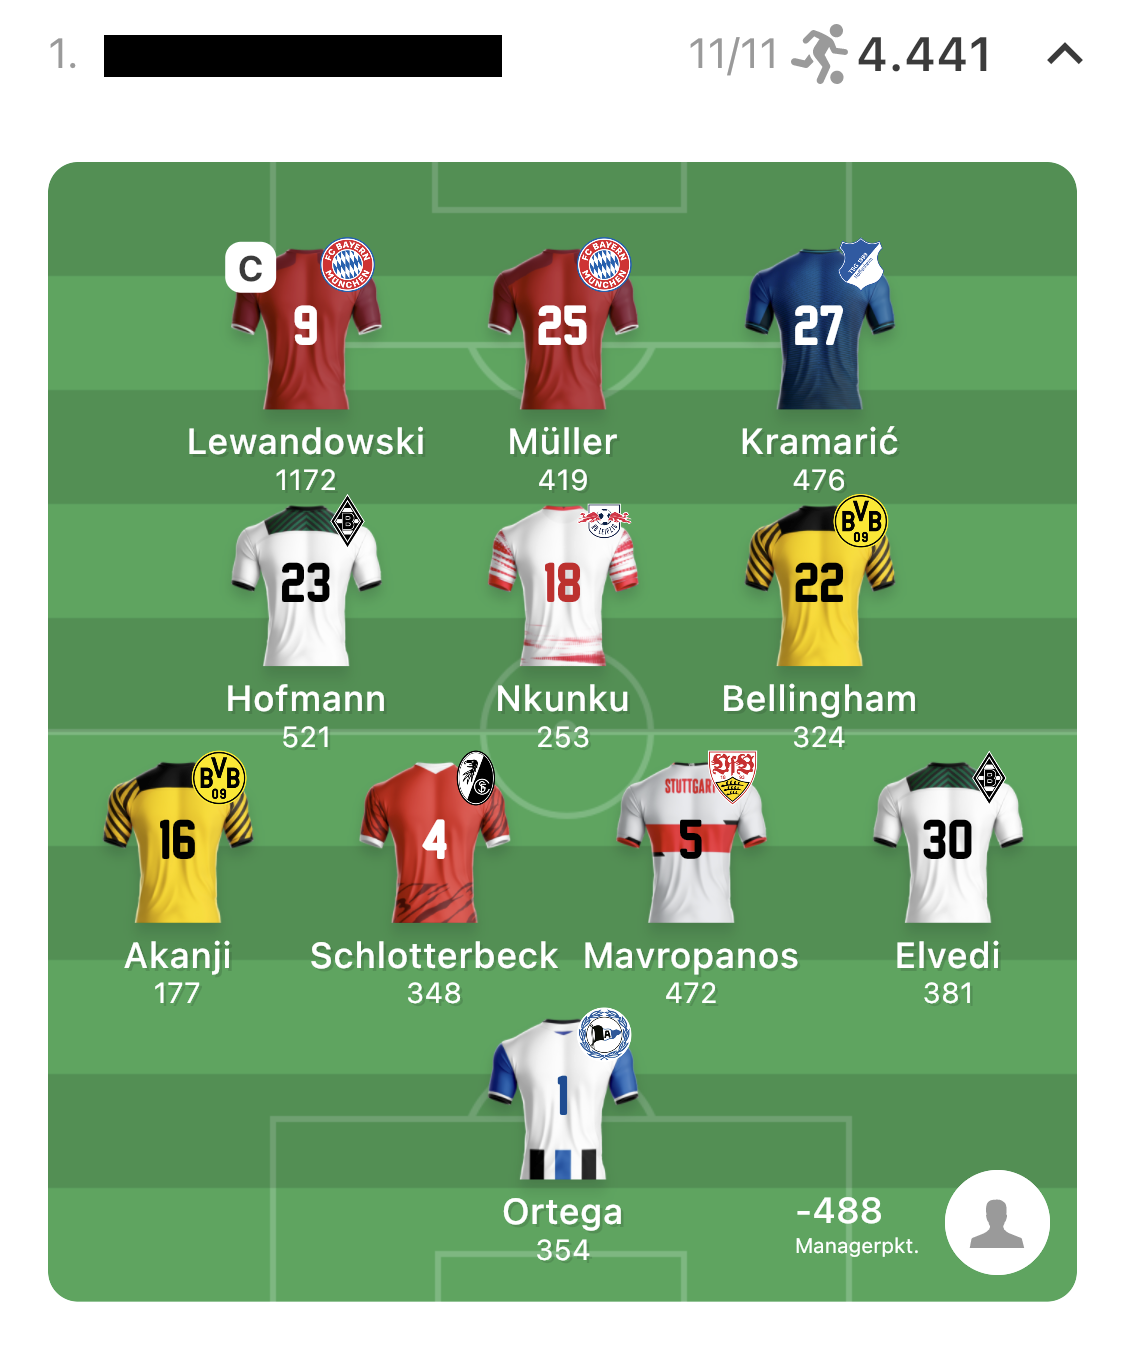
\includegraphics[width=.38\textwidth]{chapter/4_implementation/figures/first_place.png}\hfill
            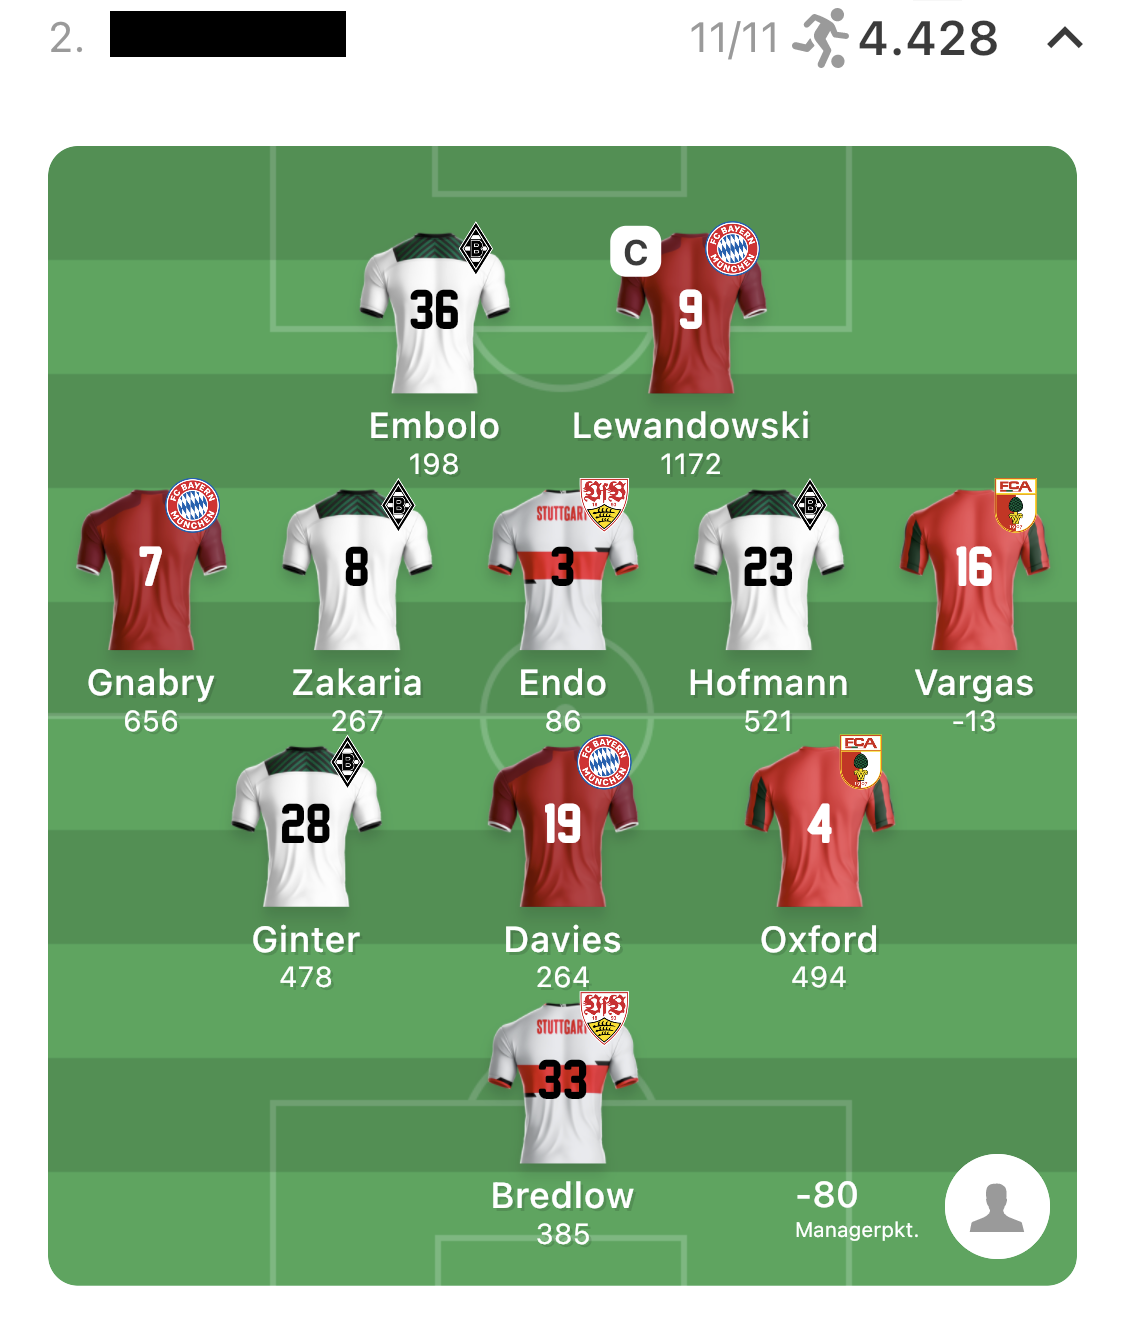
\includegraphics[width=.38\textwidth]{chapter/4_implementation/figures/second_place.png}\hfill
            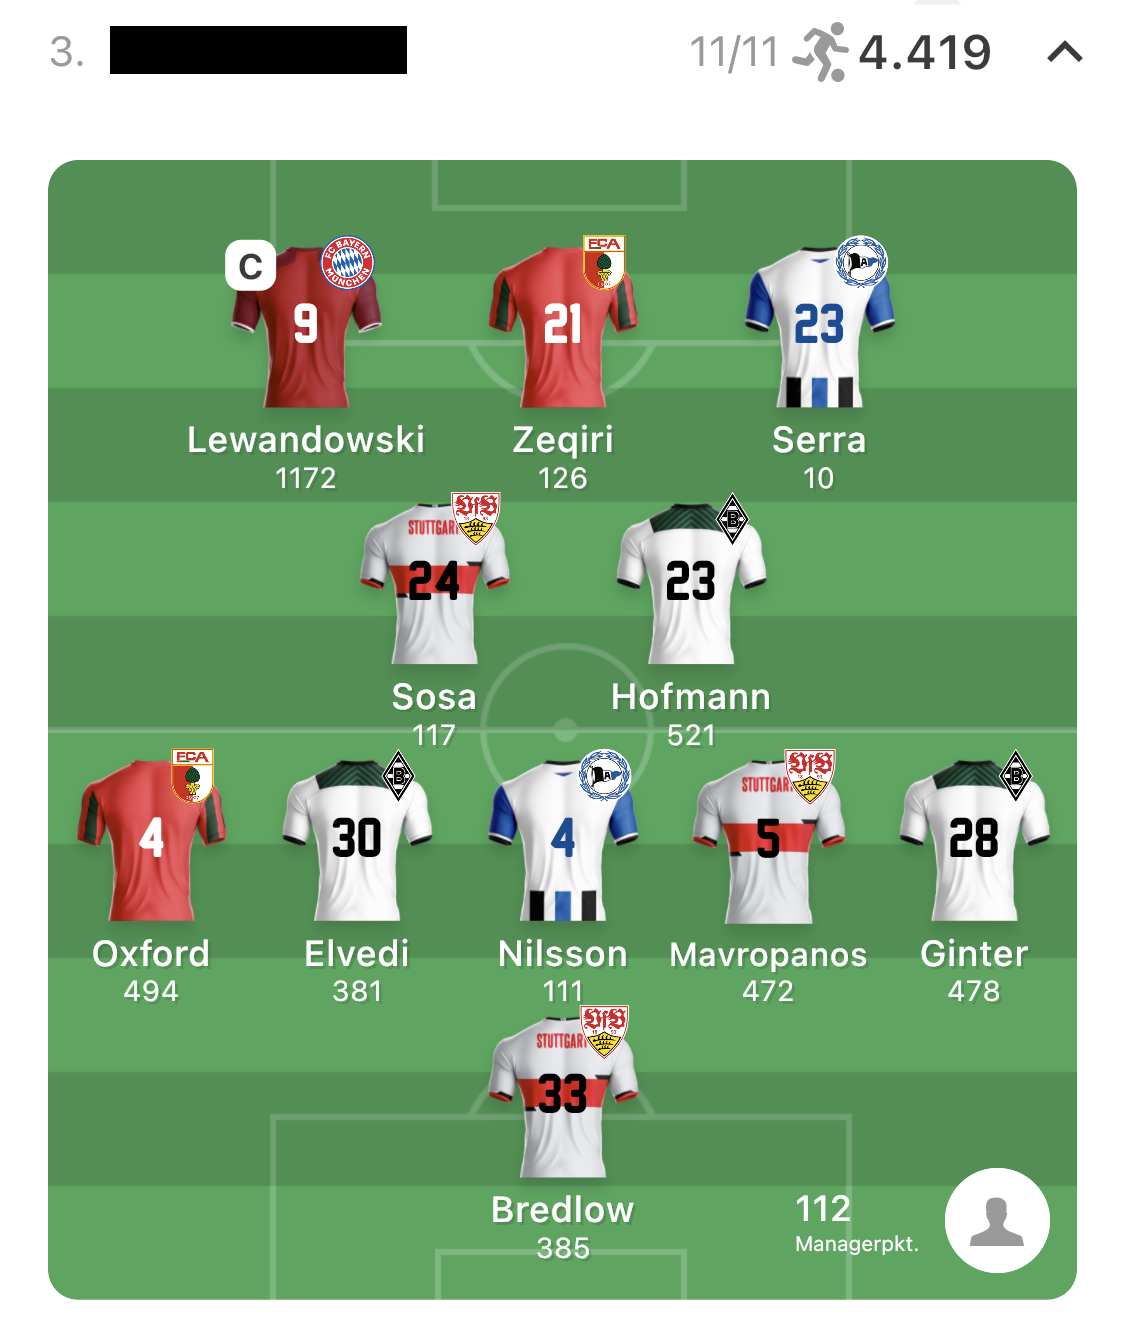
\includegraphics[width=.38\textwidth]{chapter/4_implementation/figures/third_place.png}
        }
    }
    \captionsetup{justification=centering}
    \caption{Line-Ups of Top 3 Managers from 8th matchday 2021/22}
    \label{fig:top-3}
\end{figure}

A line-up can already be assembled from the players of the best three managers, which is far better than rank one on this matchday. The best line-up from the presented players would have been:

\begin{quote}
    \centering
    Formation:  5-2-3 \\
    Captain:    Gnabry \\

    Lewandowski (586), Kramaric (476), Müller (419) \\
    Gnabry (1312), Hofmann (521) \\
    Oxford (494), Ginter (478), Mavropanos (472), Elvedi (381), Schlotterbeck (348) \\
    Bredlow (385)

    Budget needed: €198.2m (-385.6 Manager Score) \\
    Total Score: \textbf{\numprint{5486}}
\end{quote}

Therefore, rank 1 in the competition reached 81\% ($\numprint{4441} \div \numprint{5486}$) of the score, which confirms the statement made earlier. Even though this is only one example, similar proportions of the scores can be seen on any other matchday.

Furthermore, it is important to notice that there are no well-known managers who regularly achieve top ranks. According to the observations made so far, it seems challenging to field the best possible team, let alone to achieve first place regularly. A probable explanation for this, which was also often stated in the literature, is the strong influence of luck due to things that are not predictable, such as injuries. Therefore, it is much more realistic to pursue the last-mentioned goal, to end in the winning zone regularly. The previous rankings reveal that the score needed to reach the winning area is lower, between 60 and 65\% of the maximum possible score. For these reasons, this work aims to write a model that regularly achieves 65\% of the best possible score.

Regarding the second-mentioned goal, the best possible score is achieved by the line-up with the highest adjusted final line-up score \emph{S\textsubscript{LM}}. To create this line-up, the eleven players with the highest adjusted player score \emph{S\textsubscript{P\textsubscript{i}M}}, which can be placed in one of the available formations, must be found. In addition, the player with the highest player score \emph{S\textsubscript{P\textsubscript{i}}} must be appointed as captain. As the actually achieved score of a player for the upcoming match day can be seen as a label for the prediction, this is \textbf{supervised machine learning}. Additionally, as the target to predict is a numerical value, this is a \textbf{regression problem}. Since the transfer market values and all possible line-ups are already known in advance, only the final score of each player has to be predicted. From another point of view, if the prediction of the final points of each player had an accuracy of 100\%, the best line-up could be calculated automatically. Therefore, it can be concluded that the model, which is supposed to achieve a regular 65\% of the best possible score, can be divided into two parts. In the first step, a machine learning model predicts the score for each player. In the second step, the best line-up is calculated based on these scores. Since no machine learning model is needed for the second step, the goal of the work can be specified further. Hence, the updated goal is to write a model that predicts upcoming individual player performances as accurately as possible to enable the system to achieve a line-up score of 65\% of the best possible score.

The literature review shows that in the context of predicting individual player performances, future predicting metrics such as betting odds have not yet been investigated. In other contexts, these kinds of metrics have already helped to improve predictions. \parencite[cf.][]{landers_machine_2017} Moreover, these values are generally considered to have a high potential in this regard. \parencite[cf.][]{wheatcroft_profiting_2020,goldstein_wisdom_2014} For this reason, the influence of betting odds will be examined more closely in this thesis. To investigate this influence, the machine learning models will first predict the players' final scores without the betting odds features. These models are called \textbf{baseline} models. Then, the models will again predict the final scores of the players with the betting odds features. These models are called \textbf{treatment} models. Finally, it can be examined which models provided the more accurate predictions and consequently which of the models compiled the better line-up as a result.

\begin{figure}[H]
    \centering
    \fbox{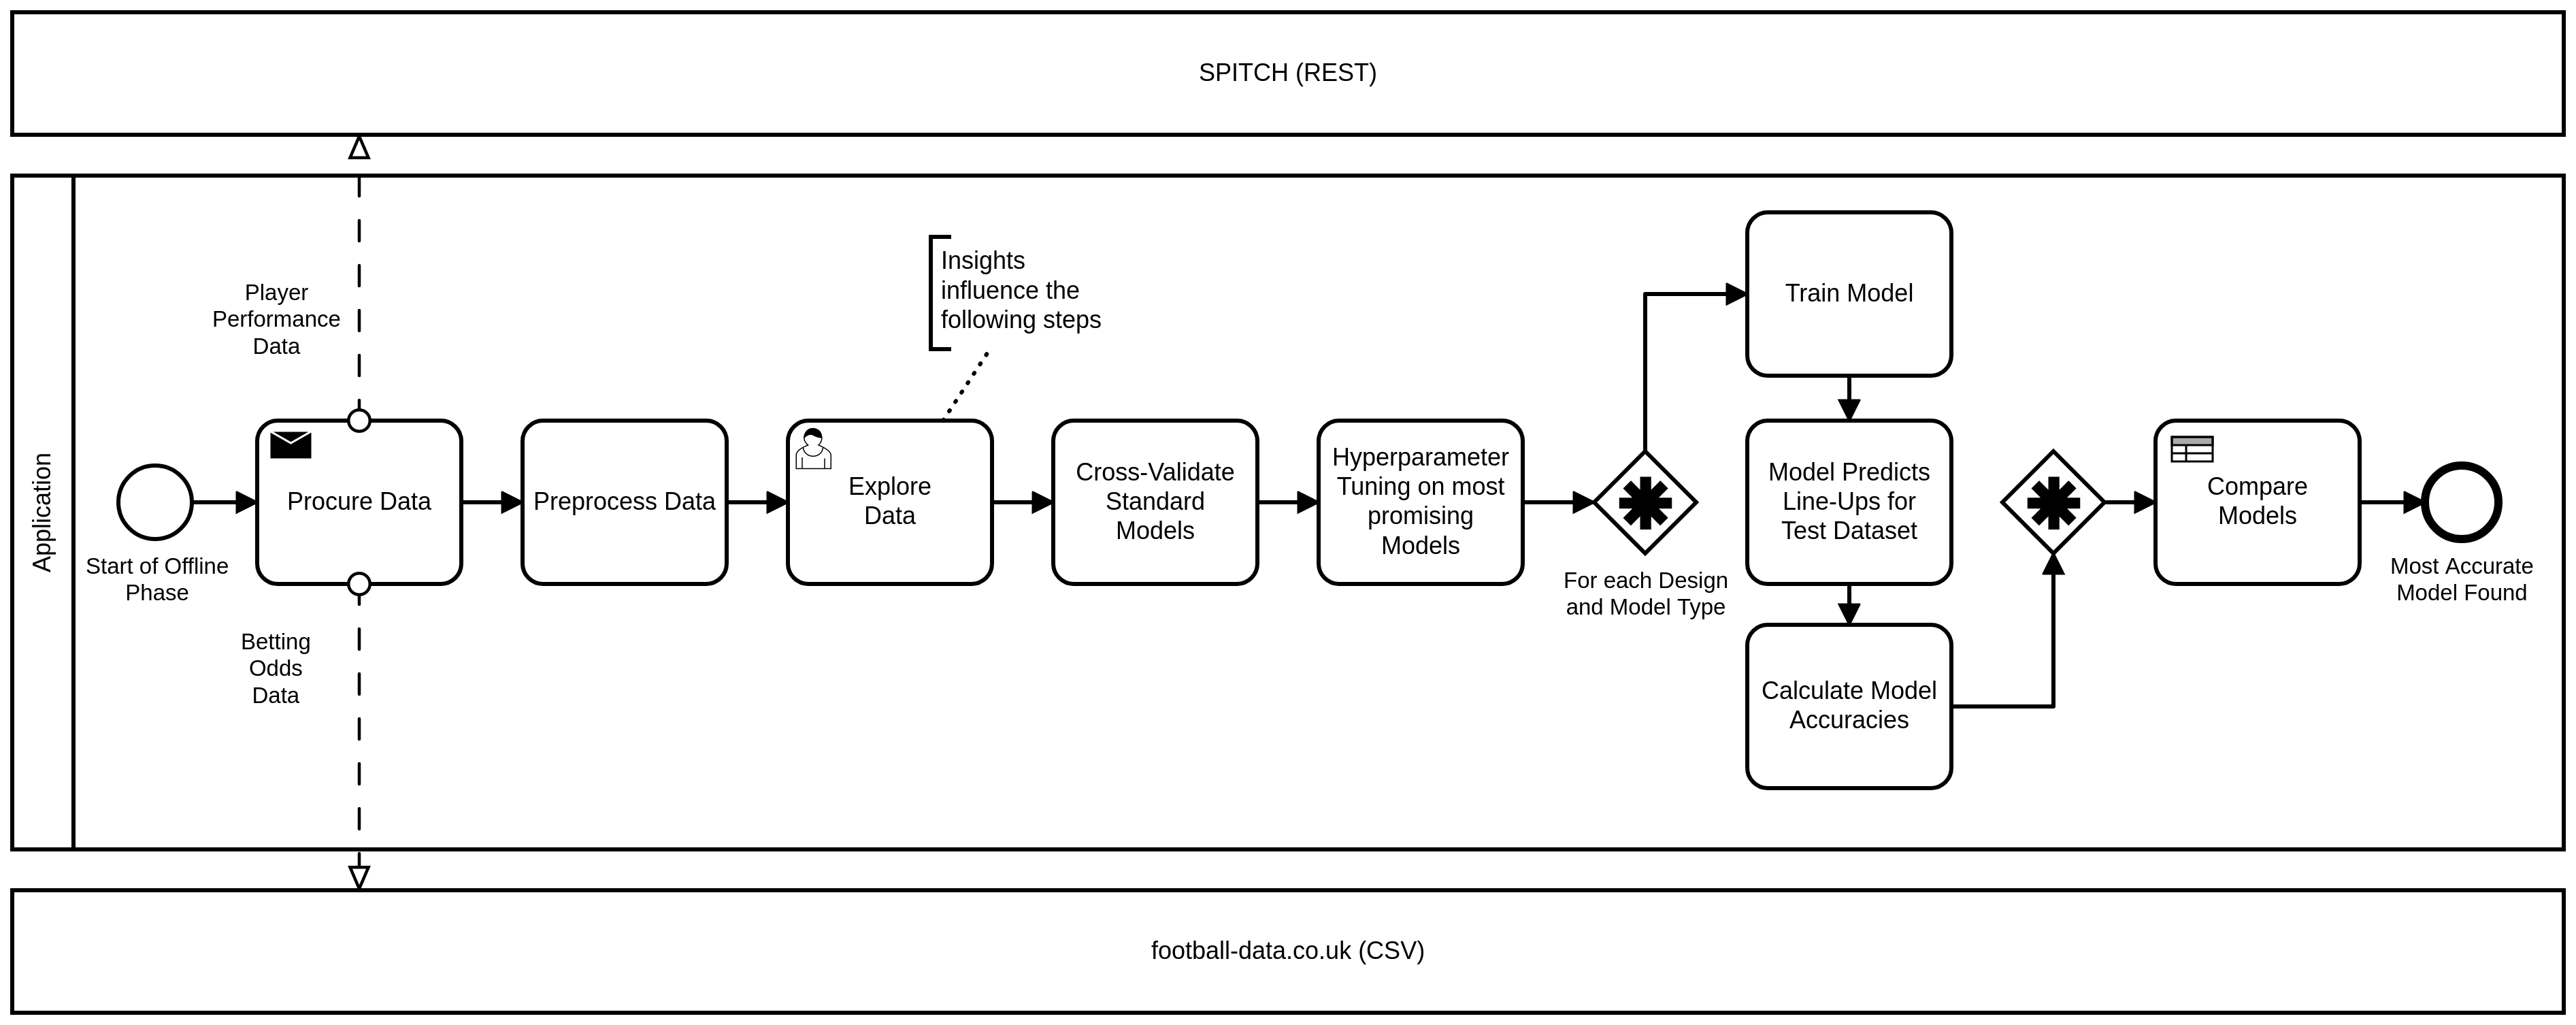
\includegraphics[width=15cm]{chapter/4_implementation/figures/offline-process.png}}
    \captionsetup{justification=centering}
    \caption{Offline Phase Process}
    \label{fig:offline-phase}
\end{figure}

From these investigations now presented, a machine learning model will emerge that provides the most accurate predictions. This model is then implemented in a tool that, prior to a matchday, collects the current and required data and feeds it to the model. Based on the model's predictions, the best line-up for the upcoming match day is created and provided to the end-user. The creation of the tool is therefore divided into two phases: an offline (see figure \ref{fig:offline-phase}) and an online phase (see figure \ref{fig:online-phase}). First, the offline phase takes place, in which the model with the most accurate predictions is found. This requires historical data. The tool can then be used in the online phase. In this phase, the next predicted line-up can be queried. For the predictions, current data is used. In \emph{Big Data} terms, the models in the offline phase are so-called batch processing models, while the model in the online phase is a stream processing model.

\begin{figure}[H]
    \centering
    \fbox{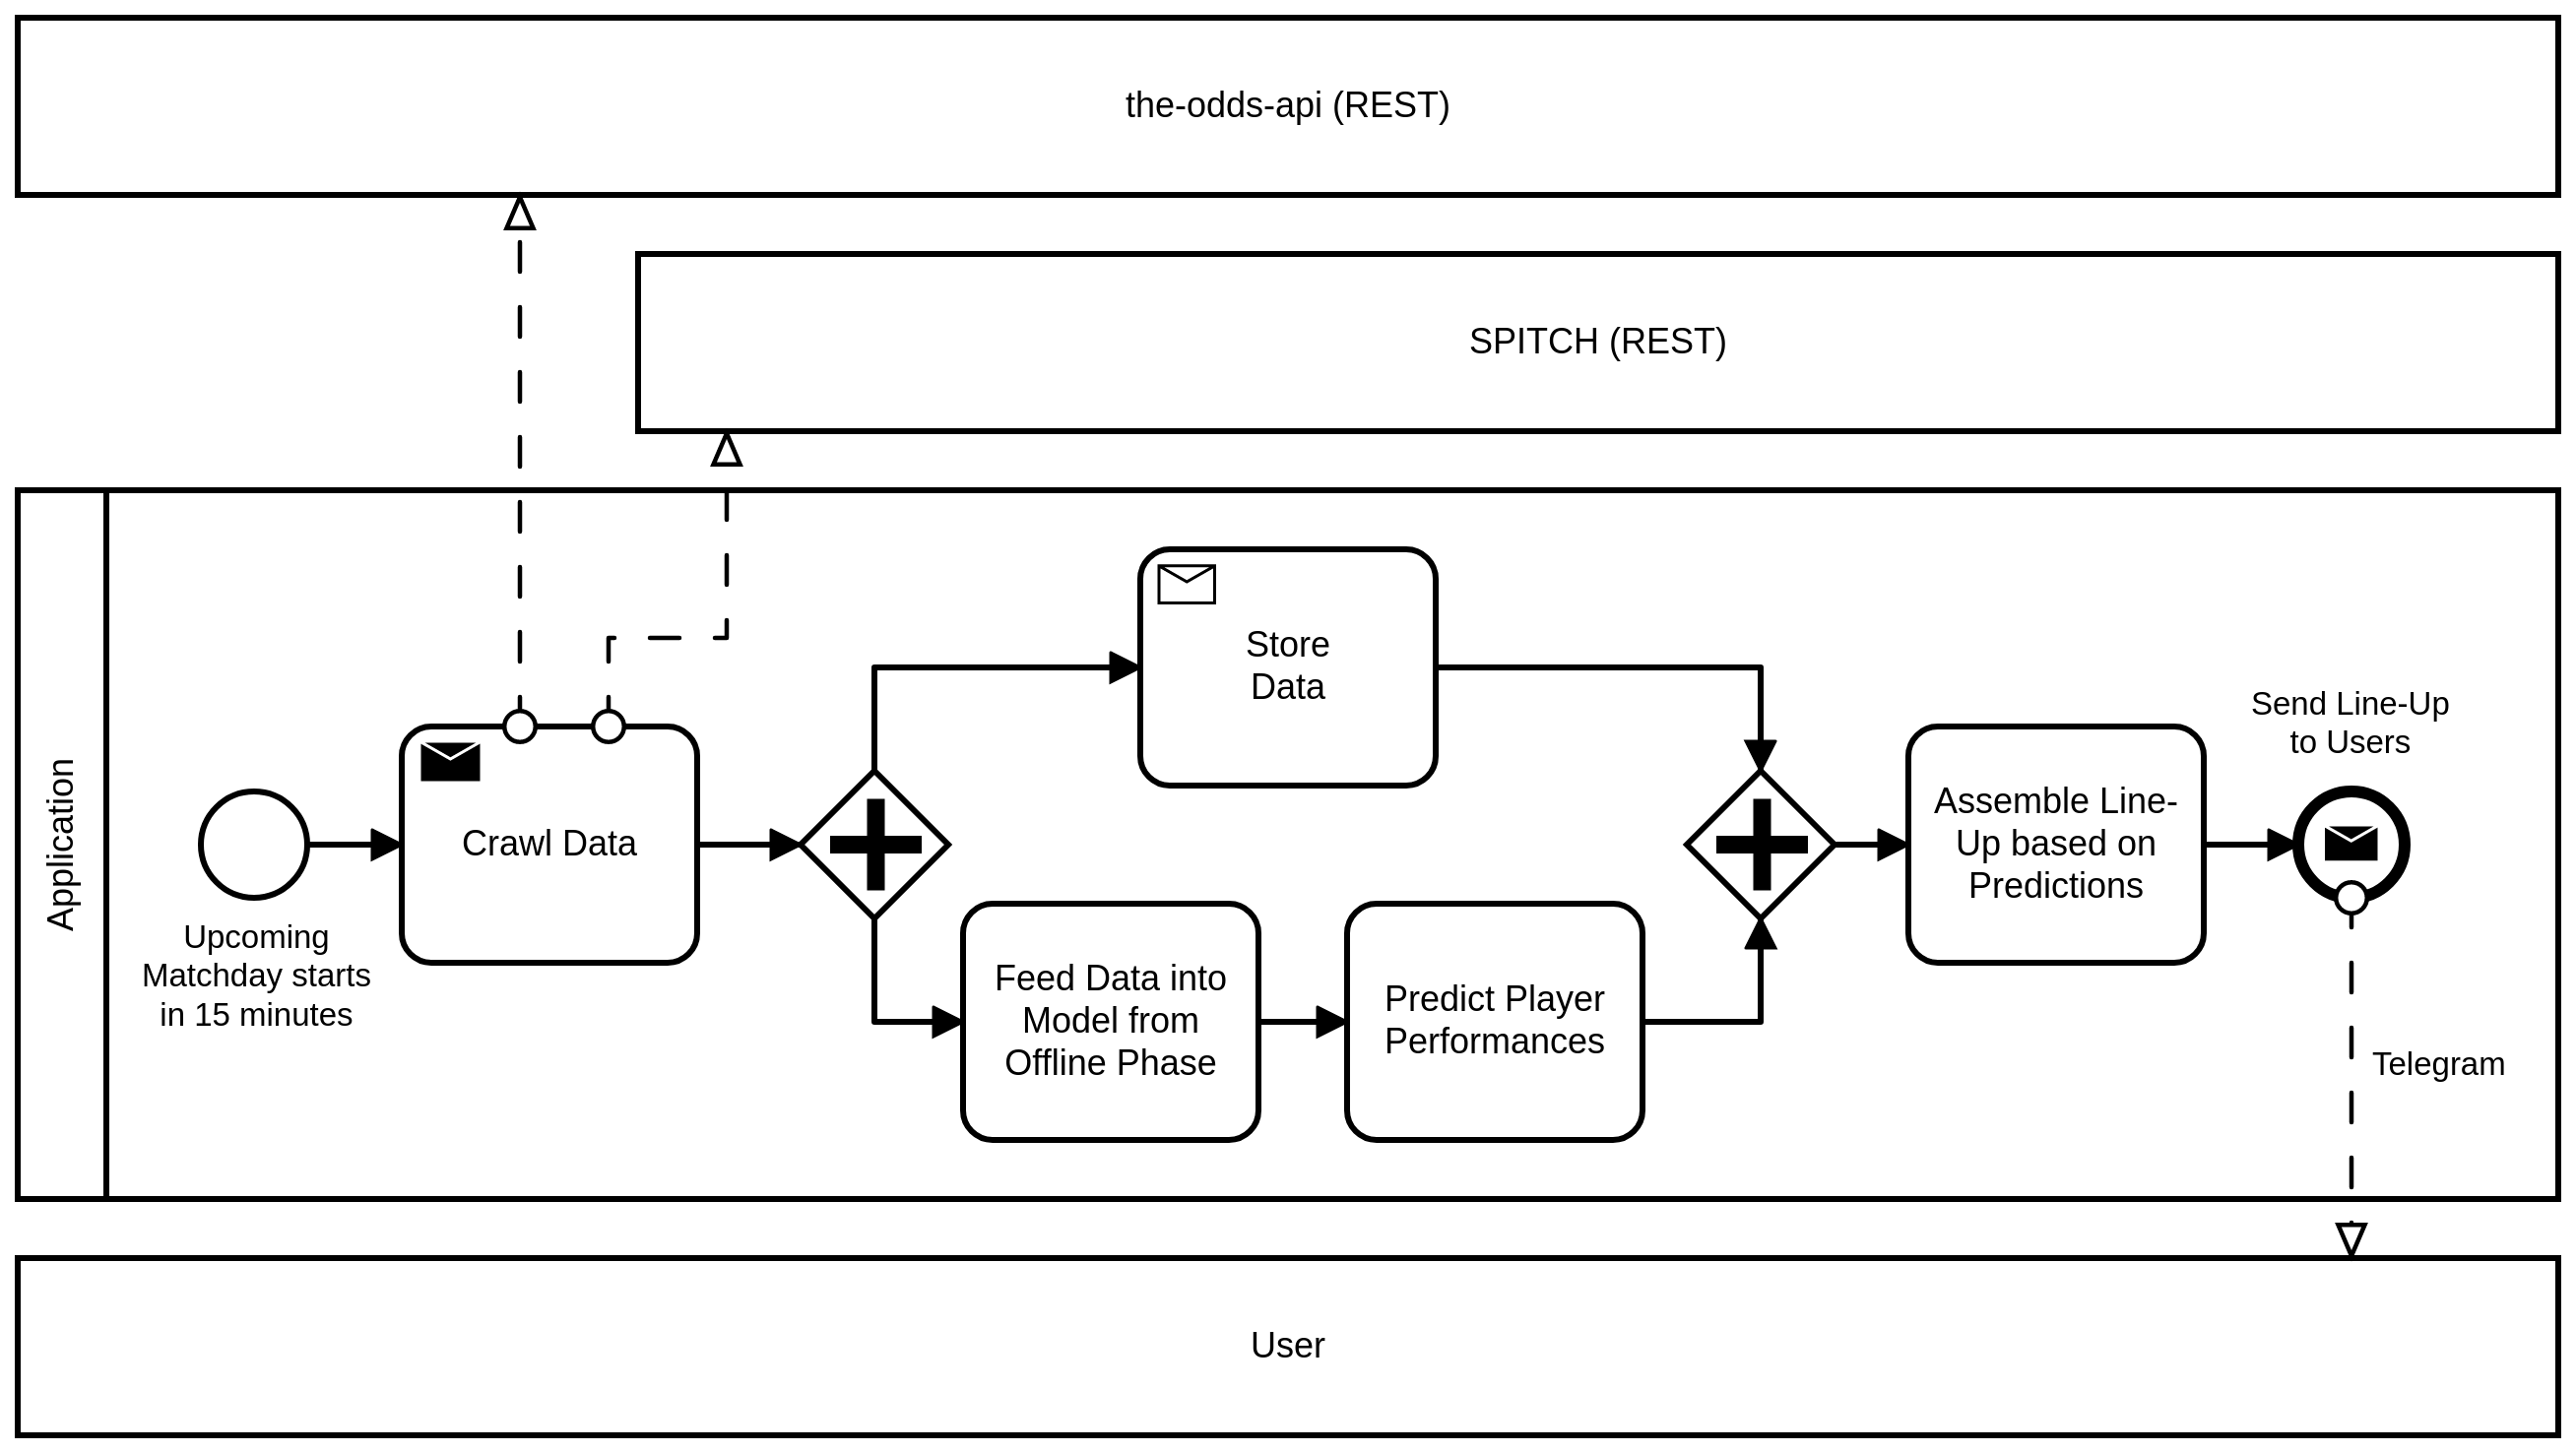
\includegraphics[width=15cm]{chapter/4_implementation/figures/online-process.png}}
    \captionsetup{justification=centering}
    \caption{Online Phase Process}
    \label{fig:online-phase}
\end{figure}

As already mentioned at the beginning of this section, SPITCH is a competition in which, on the one hand, even the best-placed players take turns and, on the other, almost never achieve the highest possible score. These two attributes are characteristics of gambling. Furthermore, football is complex and has many influencing factors that cannot all be taken into account. The betting odds try to take some of these factors into consideration, which is why they should probably lead to better results. However, it may also be that the bettors' assessment of bias is inferior. For all these reasons, it can be assumed that it is probably difficult to achieve the set target. 
